\documentclass[11pt,letterpaper]{article}
\usepackage[utf8]{inputenc}
\usepackage[T1]{fontenc}
\usepackage{lmodern}
\IfFileExists{spanish.ldf}{\usepackage[spanish,es-noshorthands,es-tabla]{babel}}{}
\usepackage[margin=2.5cm]{geometry}
\usepackage{graphicx}
\usepackage{tabularx,booktabs}
\usepackage{xcolor}
\usepackage{enumitem}
\usepackage{fancyhdr}
\usepackage{caption}
\usepackage{textcomp}
\usepackage{listings}
\usepackage{tikz}
\usetikzlibrary{positioning,arrows.meta}
\usepackage[hidelinks]{hyperref}

%% Nombres en español si no está babel-spanish (compilación local)
\makeatletter
\@ifpackageloaded{babel}{}{%
  \renewcommand{\contentsname}{Índice}
  \renewcommand{\tablename}{Tabla}
  \renewcommand{\figurename}{Figura}
  \renewcommand{\refname}{Referencias}
  \renewcommand{\abstractname}{Resumen}
  \renewcommand{\appendixname}{Anexo}}
\makeatother

%% Datos pendientes de completar: aparecen en rojo en el PDF
\newcommand{\pend}[1]{\textcolor{red}{[#1]}}
%% Referencia al Log File del proyecto
\newcommand{\logref}[1]{\textit{(Log File, #1)}}

\definecolor{codebg}{gray}{0.95}
\lstset{basicstyle=\ttfamily\small, backgroundcolor=\color{codebg},
  frame=single, rulecolor=\color{gray!50}, breaklines=true,
  columns=fullflexible, keepspaces=true, showstringspaces=false, upquote=true}

\pagestyle{fancy}
\fancyhf{}
\lhead{\small Proyecto IK-Dron}
\rhead{\small Reporte técnico}
\cfoot{\thepage}
\setlength{\headheight}{14pt}

\begin{document}

%% ============================== PORTADA ==============================
\begin{titlepage}
\centering
{\large Universidad Autónoma de Aguascalientes\par}
{\normalsize Departamento de Sistemas Electrónicos\par}
\vspace{3.5cm}
{\Huge\bfseries IK-Dron\par}
\vspace{0.5cm}
{\Large Desarrollo y puesta en vuelo de un dron de carreras\\ de 5 pulgadas con BetaFlight\par}
\vspace{0.8cm}
{\large Reporte técnico\par}
\vspace{3cm}
{\large Contreras R. Orlando\\ Garcia B. Iker\par}
\vspace{1cm}
{\normalsize \textbf{Asesor:} Dr. Luis Antonio Raygoza Pérez\par}
\vfill
{\normalsize Aguascalientes, Ags., octubre de 2026\par}
\end{titlepage}

%% ============================== RESUMEN ==============================
\begin{abstract}
Este documento describe el desarrollo del proyecto IK-Dron, un dron aéreo de carreras de 5 pulgadas construido sobre el frame LS210. El proyecto inició con una controladora CC3D programada con LibrePilot, la cual sufrió una falla irreparable en su microcontrolador. Esto motivó la migración a una controladora SpeedyBee F405 V4 con firmware BetaFlight. Se presentan la arquitectura del sistema, sus especificaciones, la configuración actual del firmware, un manual de operación, los problemas encontrados durante la puesta en vuelo junto con su solución, y los procedimientos de seguridad derivados de las pruebas. Como resultado, el dron logró un vuelo estable el 13 de octubre de 2026 en modo de autonivelado y, posteriormente, se actualizó a BetaFlight 2026.6.2 para incorporar el mantenimiento automático de altura (\textit{altitude hold}) con el barómetro de la controladora. El registro detallado, día por día, de las actividades se encuentra en el documento complementario \textit{IK-Dron Log File}, al cual se hace referencia a lo largo de este reporte.

\vspace{0.5em}
\noindent\textbf{Palabras clave:} Drone, BetaFlight, Control PID, SpeedyBee F405 V4.
\end{abstract}

\tableofcontents
\newpage

%% ============================== 1 ==============================
\section{Introducción}
Los drones de carreras (\textit{FPV racing}) son multirrotores ligeros diseñados para alcanzar altas velocidades y maniobrabilidad. Su funcionamiento depende de una controladora de vuelo que lee los sensores inerciales, ejecuta un lazo de control PID varias miles de veces por segundo y envía los comandos de velocidad a los motores a través de los controladores electrónicos de velocidad (ESC).

El proyecto IK-Dron tiene como propósito comprender y documentar cada uno de los componentes que conforman un dron de carreras, configurarlo para lograr un vuelo estable y, posteriormente, evaluar si es rentable construirlo frente a adquirir un dron comercial ya armado.

Este reporte funciona como la descripción general del proyecto. Cada sección indica entre paréntesis la sección correspondiente del \textit{Log File}, donde se encuentran las evidencias fotográficas, los incidentes y el detalle de cada sesión de trabajo.

%% ============================== 2 ==============================
\section{Objetivos}
\subsection{Objetivo general}
Mejorar, configurar y documentar el dron de carreras de 5 pulgadas capaz de realizar un vuelo estable y seguro.

\subsection{Objetivos específicos}
\begin{itemize}[nosep]
    \item Migrar la controladora de vuelo a una plataforma compatible con BetaFlight.
    \item Configurar el receptor, los motores, los modos de vuelo y el lazo de control PID.
    \item Establecer procedimientos de seguridad y una guía de solución de problemas.
    \item Documentar la operación completa del dron para futuros usuarios.
\end{itemize}

%% ============================== 3 ==============================
\section{Descripción del sistema}
\subsection{Arquitectura}
La figura \ref{fig:arquitectura} muestra la arquitectura del dron. La batería LiPo alimenta al ESC 4 en 1, que a su vez alimenta a los cuatro motores y a la controladora de vuelo. La controladora recibe los comandos del piloto a través del receptor (protocolo IBUS) y envía al ESC la velocidad de cada motor mediante el protocolo digital DShot300.


\begin{figure}[!ht]
\centering
    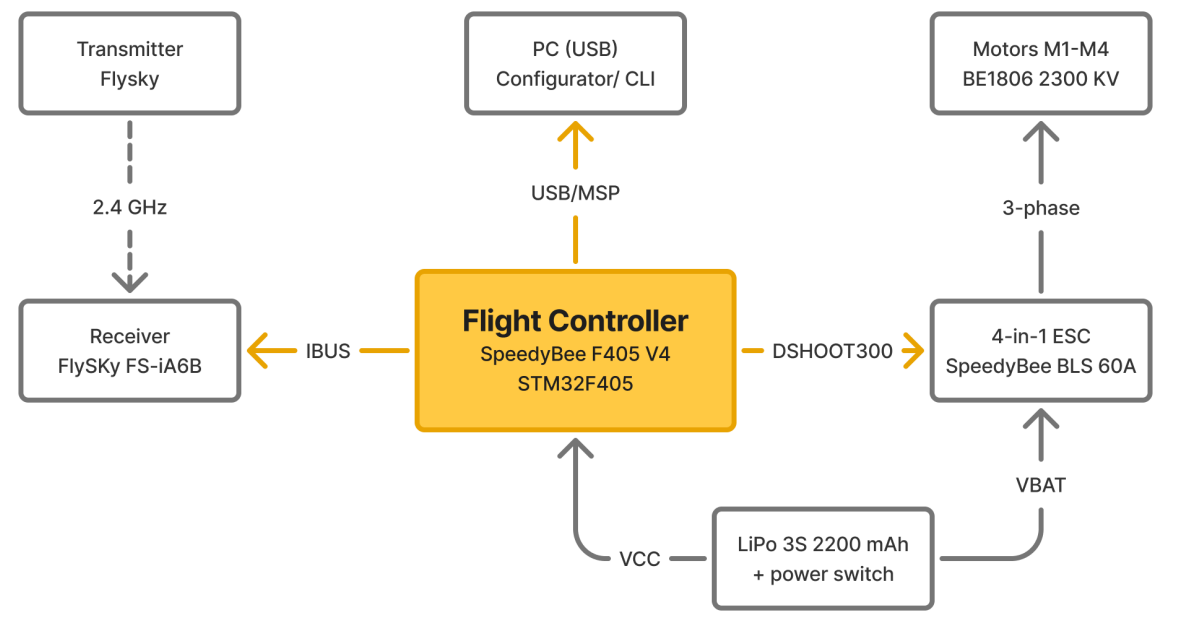
\includegraphics[width=0.6\linewidth]{src/srclog/Schematic.png}
\caption{Arquitectura del sistema IK-Dron}
\label{fig:arquitectura}
\end{figure}

\subsection{Especificaciones generales}
La tabla \ref{tab:specs} resume los componentes principales del dron. El frame, los motores, la batería y el receptor son los seleccionados por la primera generación del proyecto \cite{reporte2021}; la controladora y el ESC corresponden al \textit{stack} SpeedyBee adquirido en 2026.
\begin{table}[!ht]
\centering
\caption{Especificaciones generales del dron}
\label{tab:specs}
\begin{tabularx}{\textwidth}{@{}lX@{}}
\toprule
\textbf{Componente} & \textbf{Especificación} \\
\midrule
Frame & LS-210, fibra de carbono 3K, 210\,mm entre ejes (diagonal motor a motor), 100\,g \\
Hélices & 5 pulgadas \\
Configuración & Cuadricóptero en X, motores con giro \textit{props out} \\
Controladora de vuelo & SpeedyBee F405 V4 (detalle en la tabla \ref{tab:fc}) \\
ESC & SpeedyBee BLS 60A 4 en 1 (incluido en el \textit{stack}), 3--6S, 8 bits (BLHeli\_S), con capacitor y cable XT60 incluidos \\
Motores & FlashHobby BE1806, 2300\,KV, 18\,g, empuje de 130\,g a 25,590\,RPM (datos del fabricante) \\
Batería & LiPo Turnigy 3S (11.1\,V), 2200\,mAh, 20--40C \\
Radiocontrol & Transmisor FlySky en modo 2 y receptor FlySky FS-iA6B (6 canales) por IBUS \\
Firmware & BetaFlight 2026.6.2 (\textit{target} \texttt{SPEEDYBEEF405V4}) \\
Peso total & 497\,g \\
\bottomrule
\end{tabularx}
\end{table}

\subsection{Controladora de vuelo}
La controladora SpeedyBee F405 V4 se adquirió como \textit{stack}, es decir, junto con su ESC 4 en 1, el cual sustituye a los cuatro ESC individuales de la primera generación. Se eligió por su compatibilidad con las versiones actuales de BetaFlight, sus sensores integrados y su bajo costo \logref{Junio 2}. Los datos de la tabla \ref{tab:fc} fueron obtenidos directamente de la controladora mediante el comando \texttt{status} de la terminal de BetaFlight.

\begin{table}[!ht]
\centering
\caption{Especificaciones de la controladora SpeedyBee F405 V4}
\label{tab:fc}
\begin{tabularx}{\textwidth}{@{}lX@{}}
\toprule
\textbf{Característica} & \textbf{Valor} \\
\midrule
Microcontrolador & STM32F405, 168\,MHz \\
Giroscopio / acelerómetro & ICM42688P, lazo de giroscopio a 8\,kHz \\
Barómetro & DPS310 (I2C), utilizado por el modo ALTHOLD \\
OSD & MAX7456 (30\,$\times$\,13 caracteres) \\
Registro de vuelo & Ranura microSD para \textit{blackbox} \\
Configuración inalámbrica & Bluetooth (aplicación SpeedyBee) \\
Montaje & 30.5\,$\times$\,30.5\,mm \\
Salidas de motor & M1: PB6, M2: PB7, M3: PB0, M4: PB1 \\
Receptor & UART2 (TX: PA2, RX: PA3) \\
\bottomrule
\end{tabularx}
\end{table}

\subsection{Orden y sentido de giro de los motores}
BetaFlight espera un orden y un sentido de giro específicos para cada motor. En este dron se utiliza la configuración \textit{props out}, mostrada en la tabla \ref{tab:motores}. Un error en el sentido de giro o en la colocación de las hélices impide el vuelo, como se describe en la sección \ref{sec:problemas}.

\begin{table}[!ht]
\centering
\caption{Orden y sentido de giro de los motores (vista superior, frente hacia arriba)}
\label{tab:motores}
\begin{tabular}{@{}lll@{}}
\toprule
\textbf{Motor} & \textbf{Posición} & \textbf{Sentido de giro} \\
\midrule
M1 & Trasero derecho & Antihorario \\
M2 & Delantero derecho & Horario \\
M3 & Trasero izquierdo & Horario \\
M4 & Delantero izquierdo & Antihorario \\
\bottomrule
\end{tabular}
\end{table}

\begin{figure}[!ht]
    \centering
    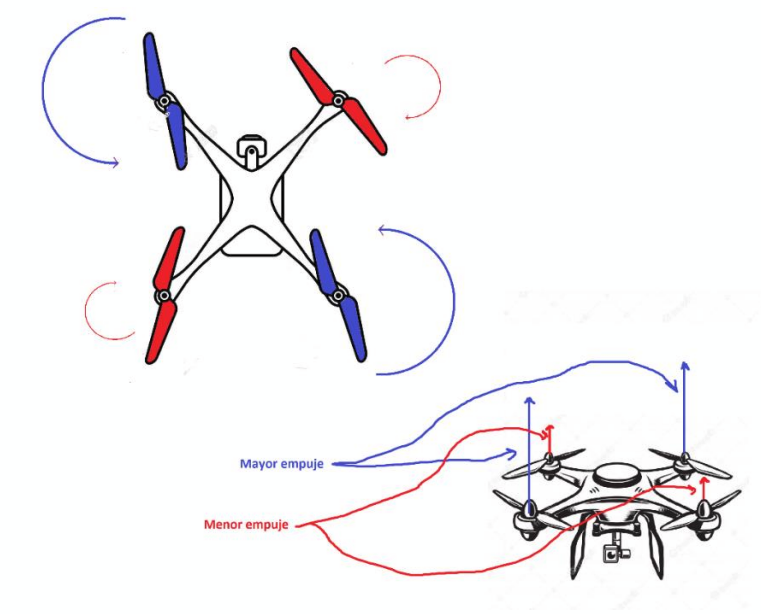
\includegraphics[width=0.6\linewidth]{src/srclog/axis.png}
    \caption{Orden de los motores}
    \label{fig:axis}
\end{figure}
%% ============================== 4 ==============================
\section{Antecedentes}
El proyecto continúa el trabajo de la primera generación (2021), realizado por Gutiérrez Castillo, Martínez Pantoja y Mares Montañez \cite{reporte2021}. En dicho trabajo se compararon distintas opciones de cada componente y se construyó el dron con los siguientes elementos:
\begin{itemize}[nosep]
    \item Frame LS-210, elegido sobre el Martian IV, ZMR250, F2 Mito GS y GEP-KX5 por su tamaño reducido, menor peso y precio.
    \item Motores FlashHobby BE1806 de 2300\,KV, por su bajo peso y precio, con un consumo aproximado de 7.6\,A por motor.
    \item Cuatro ESC FlashHobby BL20A Mini de 20\,A y una placa de distribución de energía (PDB) Lantian V3.
    \item Batería LiPo Turnigy 3S de 2200\,mAh, con la que ya se contaba.
    \item Controladora CC3D con LibrePilot, en modo Acro, con el receptor FS-iA6B conectado por PWM.
\end{itemize}
También se diseñó y fabricó una controladora propia basada en un STM32F446RE, la cual se descartó porque su costo resultaba mayor que el de una controladora comercial.

\section{Desarrollo del proyecto}
\subsection{Etapa 1: CC3D y LibrePilot (marzo -- mayo 2026)}
El dron se recibió con una controladora CC3D (microcontrolador STM32F103) programada con LibrePilot \logref{Marzo 13}. En esta etapa se aprendió el manejo básico del dron, se establecieron las primeras reglas de seguridad y se consiguió el permiso para realizar las pruebas en el estadio de la universidad \logref{Marzo 27}. También se incorporó un interruptor en la línea de la batería y se reparó una antena dañada por una caída \logref{1 de Abril}.

En abril la controladora dejó de aceptar configuraciones. Se intentó recuperarla mediante la actualización del firmware, comunicación serial \logref{10 de Abril} y finalmente un \textit{hard reset} por SWD soldando cables directamente al conector de programación \logref{15 y 27 de Mayo}. No fue posible comunicarse con el microcontrolador, por lo que se concluyó que la placa se había quemado.

\subsection{Etapa 2: migración a BetaFlight (junio -- agosto 2026)}
Dado que las versiones actuales de BetaFlight ya no soportan los microcontroladores de la familia F1, se decidió reemplazar la CC3D por una controladora moderna. Se investigaron las opciones disponibles y se eligió la SpeedyBee F405 V4, adquirida en AliExpress \logref{Junio 2}. La controladora se instaló en el frame, se conectó el receptor por IBUS y se actualizó a BetaFlight 4.4.3 \logref{Agosto 28}.

\subsection{Etapa 3: puesta en vuelo (septiembre -- octubre 2026)}
Durante varios intentos el dron no logró volar: primero no levantaba y, tras invertir el giro de los motores, despegaba con un brinco y se desarmaba \logref{Septiembre}. En octubre se realizó un diagnóstico completo desde la terminal de BetaFlight, se identificaron las causas (sección \ref{sec:problemas}), se corrigió la configuración y el dron logró un vuelo estable \logref{7 a 13 de Octubre}.

\subsection{Etapa 4: mantenimiento automático de altura (octubre 2026)}
Para que el dron pueda flotar a una altura constante sin que el piloto corrija el acelerador, se actualizó el firmware a BetaFlight 2026.6.2, que incorpora el modo ALTHOLD. Este modo utiliza el barómetro DPS310 de la controladora para medir la altura. Al no contar con GPS, el dron mantiene la altura pero no su posición horizontal. Debido a que el configurador web no lograba poner la controladora en modo DFU, el firmware se grabó desde la terminal con \texttt{dfu-util} (anexo \ref{anx:flash}) y la configuración se volvió a aplicar por la CLI \logref{23 de Octubre}.

%% ============================== 5 ==============================
\section{Configuración actual}
La configuración se orientó a un vuelo suave y fácil de controlar, adecuado para pilotos principiantes. La tabla \ref{tab:config} resume los parámetros principales; los valores no listados se encuentran en los valores por defecto de BetaFlight 2026.6.2. El respaldo completo se encuentra en la carpeta \texttt{respaldos} del proyecto.

\begin{table}[!ht]
\centering
\caption{Parámetros principales de BetaFlight 2026.6.2}
\label{tab:config}
\begin{tabularx}{\textwidth}{@{}llX@{}}
\toprule
\textbf{Parámetro} & \textbf{Valor} & \textbf{Descripción} \\
\midrule
\texttt{serialrx\_provider} & IBUS & Protocolo del receptor (UART2) \\
\texttt{map} & AETR & Orden de canales del radio \\
\texttt{motor\_pwm\_protocol} & DSHOT300 & Protocolo digital hacia los ESC \\
\texttt{dshot\_bidir} & OFF & Sin telemetría de RPM \\
\texttt{yaw\_motors\_reversed} & ON & Configuración \textit{props out} \\
\texttt{feature MOTOR\_STOP} & Activo & Los motores no giran armado con el acelerador en cero \\
Armado & AUX1, 1950--2075 & Interruptor de armado \\
Modo ANGLE & Siempre activo & Autonivelado: al soltar los sticks el dron se nivela \\
Modo ALTHOLD & AUX2, 1700--2100 & Mantiene la altura con el barómetro \\
\texttt{angle\_limit} & 30° & Inclinación máxima en modo ANGLE \\
\texttt{small\_angle} & 25° & No permite armar si el dron está inclinado \\
\texttt{runaway\_takeoff\_prevention} & ON & Desarma si el dron se descontrola al despegar \\
\texttt{failsafe\_procedure} & DROP & Si pierde la señal por 1.5\,s, apaga los motores \\
\texttt{ap\_hover\_throttle} & 1275 & Acelerador estimado para flotar (por ajustar) \\
Perfil PID / Rates & 0 / 0 & Perfiles activos \\
Filtros & Por defecto & Ajustados para operar sin filtro RPM \\
\bottomrule
\end{tabularx}
\end{table}

\newpage
\subsection{Ganancias PID}
Se utilizan las ganancias por defecto de BetaFlight 2026.6.2, que son las mismas de la versión 4.4 y están diseñadas para drones de 5 pulgadas (tabla \ref{tab:pid}). Estas servirán como punto de partida para la sintonización con base en los registros del \textit{blackbox}.

\begin{table}[!ht]
\centering
\caption{Ganancias PID (perfil 0)}
\label{tab:pid}
\begin{tabular}{@{}lccccc@{}}
\toprule
\textbf{Eje} & \textbf{P} & \textbf{I} & \textbf{D} & \textbf{D máx} & \textbf{FF} \\
\midrule
Roll  & 45 & 80 & 30 & 40 & 120 \\
Pitch & 47 & 84 & 34 & 46 & 125 \\
Yaw   & 45 & 80 & 0  & 0  & 120 \\
\bottomrule
\end{tabular}
\end{table}

\subsection{Rates}
Se redujeron las tasas de giro (\textit{rates}, tipo \textit{Actual}) para obtener una respuesta suave a los sticks (tabla \ref{tab:rates}).

\begin{table}[!ht]
\centering
\caption{Rates configurados (perfil 0)}
\label{tab:rates}
\begin{tabular}{@{}lccc@{}}
\toprule
\textbf{Eje} & \textbf{Centro (°/s)} & \textbf{Máximo (°/s)} & \textbf{Expo} \\
\midrule
Roll / Pitch & 40 & 300 & 0.40 \\
Yaw          & 40 & 250 & 0.30 \\
\bottomrule
\end{tabular}
\end{table}

Antes de cualquier cambio se recomienda guardar un respaldo de la configuración con el comando \texttt{diff all} (anexo \ref{anx:cli}).

%% ============================== 6 ==============================
\section{Manual de operación}
\label{sec:manual}
Esta sección describe cómo utilizar el dron desde la preparación de la batería hasta el apagado. Se recomienda leerla completa antes del primer vuelo junto con los procedimientos de seguridad (sección \ref{sec:seguridad}).

\subsection{Controles del transmisor}
El transmisor se utiliza en modo 2. La tabla \ref{tab:controles} indica la función de cada control.

\begin{table}[!ht]
\centering
\caption{Controles del transmisor (modo 2)}
\label{tab:controles}
\begin{tabularx}{\textwidth}{@{}llX@{}}
\toprule
\textbf{Control} & \textbf{Canal} & \textbf{Función} \\
\midrule
Stick izquierdo, arriba/abajo & Throttle & Acelerador: sube o baja el dron \\
Stick izquierdo, izquierda/derecha & Yaw & Gira el dron sobre su propio eje \\
Stick derecho, arriba/abajo & Pitch & Inclina el dron hacia adelante o hacia atrás \\
Stick derecho, izquierda/derecha & Roll & Inclina el dron hacia los lados \\
Interruptor del canal 5 & AUX1 & Armado: arriba arma los motores, abajo los desarma \\
Interruptor del canal 6 & AUX2 & ALTHOLD: arriba mantiene la altura, abajo vuelo normal \\
\bottomrule
\end{tabularx}
\end{table}

Los interruptores de los canales 5 y 6 se asignan en el menú \textit{Functions setup} $\rightarrow$ \textit{Aux. channels} del transmisor FlySky. Ambos deben estar abajo antes de encender el dron.

\subsection{Batería}
La batería es una LiPo de 3 celdas (3S). Cada celda tiene un voltaje nominal de 3.7\,V; la tabla \ref{tab:bateria} muestra los voltajes de referencia.

\begin{table}[!ht]
\centering
\caption{Voltajes de referencia de la batería LiPo 3S}
\label{tab:bateria}
\begin{tabular}{@{}lcc@{}}
\toprule
\textbf{Estado} & \textbf{Por celda} & \textbf{Total (3S)} \\
\midrule
Carga completa & 4.20\,V & 12.6\,V \\
Almacenamiento (si no se usará en días) & 3.80\,V & 11.4\,V \\
Alerta de BetaFlight: aterrizar & 3.50\,V & 10.5\,V \\
Mínimo absoluto, no descargar por debajo & 3.30\,V & 9.9\,V \\
\bottomrule
\end{tabular}
\end{table}

\begin{itemize}[nosep]
    \item Cargar siempre con un cargador balanceador y bajo supervisión.
    \item Antes de volar, revisar el voltaje de cada celda con el checador \logref{Marzo 13}. Las tres celdas deben tener voltajes similares (diferencia menor a 0.1\,V).
    \item No utilizar una batería inflada o golpeada.
\end{itemize}

\subsection{Encendido}
\begin{enumerate}[nosep]
    \item Encender primero el transmisor, con el acelerador al mínimo y los interruptores AUX1 y AUX2 abajo.
    \item Colocar el dron en una superficie plana, lejos de personas.
    \item Conectar la batería o activar el interruptor de energía sujetando el dron contra el suelo \logref{Marzo 13}.
    \item Esperar los tonos de inicio de los ESC y no mover el dron durante unos segundos, ya que la controladora calibra el giroscopio al encender.
\end{enumerate}

\subsection{Armado y despegue}
\begin{enumerate}[nosep]
    \item Con el acelerador al mínimo, subir el interruptor AUX1 para armar.
    \item \textbf{Importante:} con la función \texttt{MOTOR\_STOP}, los motores no giran aunque el dron esté armado si el acelerador está en cero. Un dron armado debe tratarse siempre como si los motores estuvieran girando.
    \item Subir el acelerador de forma suave hasta que el dron despegue y estabilizarlo a una altura de 1 a 2\,m.
\end{enumerate}
Si el dron no arma, revisar las banderas de armado (sección \ref{sec:problemas}). Las causas más comunes son que el acelerador no está al mínimo, que el dron está inclinado más de 25° o que no hay señal del transmisor.

\subsection{Vuelo en modo ANGLE}
El modo ANGLE está siempre activo. En este modo el stick derecho controla el ángulo de inclinación del dron (máximo 30°) y, al soltarlo, el dron regresa a la posición nivelada. El acelerador controla la altura y el stick izquierdo horizontal gira el dron. Se recomienda realizar movimientos pequeños y suaves, y mantener el dron siempre a la vista.

\subsection{Mantenimiento de altura (ALTHOLD)}
\begin{enumerate}[nosep]
    \item Despegar y estabilizar el dron a una altura de 1 a 2\,m en vuelo normal.
    \item Subir el interruptor AUX2. El dron mantendrá la altura en la que se encontraba.
    \item Colocar el acelerador en el centro. Moverlo hacia arriba o abajo hace que el dron suba o baje de forma controlada, y al regresarlo al centro mantiene la nueva altura.
    \item El dron no mantiene su posición horizontal: el viento lo desplaza, por lo que se debe corregir con el stick derecho.
    \item Si el dron sube, baja u oscila de forma brusca, bajar el interruptor AUX2 de inmediato y retomar el control con el acelerador.
\end{enumerate}

\subsection{Aterrizaje y apagado}
\begin{enumerate}[nosep]
    \item Si ALTHOLD está activo, bajar el interruptor AUX2.
    \item Bajar el acelerador suavemente hasta que el dron toque el suelo.
    \item Llevar el acelerador al mínimo y bajar el interruptor AUX1 para desarmar.
    \item Desconectar la batería o apagar el interruptor de energía. Apagar el transmisor siempre al final.
\end{enumerate}

\subsection{Emergencias}
\begin{itemize}[nosep]
    \item \textbf{Pérdida de control:} bajar el interruptor AUX1. Los motores se detienen de inmediato y el dron cae, por lo que se debe hacer cuando el dron está a baja altura o en una zona despejada.
    \item \textbf{Pérdida de señal:} si el dron deja de recibir la señal del transmisor por 1.5\,s, apaga los motores y cae (\textit{failsafe} en modo DROP). Por ello se debe volar siempre dentro del alcance del transmisor.
    \item \textbf{Brinco al despegar y desarmado:} es la protección \textit{Runaway Takeoff}. No se debe volver a intentar el vuelo hasta revisar las hélices y el sentido de giro de los motores.
\end{itemize}

\subsection{Después del vuelo}
\begin{itemize}[nosep]
    \item Revisar la temperatura de los motores con la mano: deben estar tibios, no calientes.
    \item Revisar que las hélices no estén dañadas y sigan apretadas.
    \item Medir el voltaje de la batería y dejarla en voltaje de almacenamiento si no se volverá a usar en los siguientes días.
\end{itemize}

\subsection{Conexión a la computadora}
\begin{itemize}[nosep]
    \item \textbf{BetaFlight Configurator:} se utiliza desde \url{https://app.betaflight.com} en Chrome o Chromium. Firefox no permite actualizar el firmware y Brave bloquea el acceso al USB por defecto.
    \item \textbf{Aplicación SpeedyBee:} permite configurar el dron por Bluetooth desde el teléfono.
    \item \textbf{Terminal:} con los scripts de Python del anexo \ref{anx:cli} se pueden consultar y modificar los parámetros directamente.
    \item Antes de probar motores desde la computadora se deben retirar las hélices. Para probar los motores o el receptor es necesario conectar la batería, ya que el USB no alimenta al ESC.
\end{itemize}

%% ============================== 7 ==============================
\section{Guía de solución de problemas}
\label{sec:problemas}
La tabla \ref{tab:problemas} reúne los problemas encontrados durante el proyecto, su causa y su solución. Las banderas (\textit{flags}) se consultan con el comando \texttt{status} en la línea \textit{Arming disable flags}, o en la pestaña \textit{Setup} del BetaFlight Configurator.

\begin{table}[!ht]
\centering
\caption{Problemas frecuentes y su solución}
\label{tab:problemas}
\small
\begin{tabularx}{\textwidth}{@{}>{\raggedright\arraybackslash}p{3.2cm}>{\raggedright\arraybackslash}X>{\raggedright\arraybackslash}X>{\raggedright\arraybackslash}p{2.1cm}@{}}
\toprule
\textbf{Síntoma} & \textbf{Causa} & \textbf{Solución} & \textbf{Log File} \\
\midrule
Los motores giran pero el dron no levanta &
Hélices colocadas al revés: empujan el aire hacia arriba &
Colocar en cada motor la hélice de su sentido de giro (borde de ataque primero) &
Sept., 7 Oct. \\
\addlinespace
Despega con un brinco y se desarma &
Protección \textit{Runaway Takeoff}: el giro de los motores no coincide con \texttt{yaw\_motors\_reversed}, o hay motores fuera de orden &
Verificar orden y giro (tabla \ref{tab:motores}). No invertir motores sin invertir también las hélices &
Sept., 7 Oct. \\
\addlinespace
Bandera \texttt{RXLOSS} &
No llega señal del receptor &
Encender el control, verificar el enlace y la alimentación del receptor &
7 Oct. \\
\addlinespace
Bandera \texttt{RPMFILTER} &
DShot bidireccional activo sin telemetría de los ESC &
Conectar la batería; si persiste, \texttt{set dshot\_bidir = OFF} &
10 Oct. \\
\addlinespace
Bandera \texttt{NO\_ACC\_CAL} &
Modo ANGLE activo con acelerómetro sin calibrar &
Calibrar el acelerómetro en superficie plana (pestaña \textit{Setup}) &
13 Oct. \\
\addlinespace
Banderas \texttt{CLI}, \texttt{MSP} o \texttt{CALIB} &
Conexión a la PC o calibración del giroscopio en curso &
Desconectar el USB; mantener el dron quieto al energizar &
13 Oct. \\
\addlinespace
El dron se carga hacia un lado &
Acelerómetro sin calibrar o desbalance físico &
Calibrar el acelerómetro; revisar hélices y centro de masa &
Marzo 27 \\
\addlinespace
No responde al movimiento lateral (roll) &
En diagnóstico: posible error en el orden físico de los motores o falta de empuje (relación empuje/peso cercana a 1:1) &
Verificar en la pestaña \textit{Motors} que cada motor corresponda a su posición (tabla \ref{tab:motores}) &
23 Oct. \\
\addlinespace
ALTHOLD sube, baja u oscila &
Acelerador de \textit{hover} mal estimado o flujo de aire sobre el barómetro &
Ajustar \texttt{ap\_hover\_throttle}; cubrir el barómetro con espuma &
23 Oct. \\
\addlinespace
El configurador no actualiza el firmware o no entra en DFU &
El navegador no soporta WebUSB (Firefox) o lo bloquea (Brave) &
Usar Chrome o Chromium, o grabar desde la terminal con \texttt{bl} y \texttt{dfu-util} (anexo \ref{anx:flash}) &
23 Oct. \\
\addlinespace
\texttt{SD card: Startup failed} &
No hay tarjeta microSD o no tiene formato válido &
Insertar microSD en formato FAT32 para el \textit{blackbox} &
13 Oct. \\
\bottomrule
\end{tabularx}
\end{table}

%% ============================== 8 ==============================
\section{Procedimientos de seguridad}
\label{sec:seguridad}
Las siguientes reglas se derivan de los incidentes registrados en el \textit{Log File}:

\noindent\textbf{Antes de volar}
\begin{enumerate}[nosep]
    \item Revisar el voltaje de cada celda de la batería con un checador, conectando negativo con negativo \logref{Marzo 13}.
    \item Verificar que las tuercas de las hélices estén apretadas \logref{Marzo 13}.
    \item Sujetar la batería y su cable lejos de las hélices \logref{Marzo 13, 1 de Abril}.
    \item Colocar los controles del radio en su posición por defecto, el acelerador en cero y los interruptores AUX1 y AUX2 abajo \logref{Marzo 13}.
    \item Volar únicamente en el estadio, lejos de salones y automóviles, sin exceder la altura permitida \logref{Marzo 27}.
\end{enumerate}

\noindent\textbf{Durante la configuración}
\begin{enumerate}[nosep]
    \item Retirar las hélices antes de probar motores desde la PC.
    \item Configurar siempre con el dron desarmado \logref{Marzo 27}.
    \item Guardar un respaldo con \texttt{diff all} antes de realizar cambios \logref{23 de Octubre}.
    \item No desactivar la protección \textit{Runaway Takeoff}.
\end{enumerate}

%% ============================== 9 ==============================
\section{Trabajo futuro}
\begin{itemize}[nosep]
    \item Realizar la prueba de vuelo del modo ALTHOLD y ajustar \texttt{ap\_hover\_throttle} con el acelerador real de \textit{hover}.
    \item Diagnosticar la falta de respuesta en roll revisando el orden de los motores y los valores enviados a cada uno.
    \item Mejorar la relación empuje/peso: el dron pesa 497\,g y los cuatro motores BE1806 producen alrededor de 520\,g de empuje según el fabricante, mientras que la primera generación recomienda al menos el doble del peso del dron \cite{reporte2021}. Se recomienda evaluar motores de mayor tamaño (por ejemplo, 2205--2207) para hélices de 5 pulgadas.
    \item Instalar una tarjeta microSD y sintonizar el PID con base en los registros del \textit{blackbox}.
    \item Limitar el acelerador y configurar el \textit{failsafe} con aterrizaje controlado.
    \item Evaluar el firmware de los ESC (Bluejay) para habilitar el DShot bidireccional y el filtro RPM.
    \item Incorporar un módulo GPS para habilitar el modo \textit{Position Hold}, ya incluido en el firmware instalado.
    \item Realizar pruebas de desempeño (tiempo de vuelo, consumo y velocidad).
\end{itemize}

%% ============================== 10 ==============================
\section{Conclusiones}
La falla de la controladora CC3D, aunque retrasó el proyecto, permitió migrar a una plataforma moderna con BetaFlight, con mejores sensores, mayor capacidad de procesamiento y herramientas de diagnóstico más completas. La terminal de BetaFlight resultó fundamental para identificar con precisión los problemas que impedían el vuelo, en lugar de realizar cambios a prueba y error, y también permitió actualizar el firmware cuando el configurador web no lo logró.

La principal lección del proyecto es que la configuración física (orden de motores, sentido de giro y colocación de hélices) debe coincidir exactamente con la configuración del firmware; un error en cualquiera de ellos se manifiesta como un dron que no levanta o que se desarma al despegar. Con la configuración actual, el dron realiza un vuelo estable y suave, cuenta con mantenimiento automático de altura, y se dispone de un manual de operación y una base documentada para continuar con la sintonización. El principal límite actual del sistema es la relación empuje/peso, que deberá mejorarse para aprovechar por completo las capacidades de la controladora.

%% ============================== REFERENCIAS ==============================
\begin{thebibliography}{9}
\bibitem{bfwiki} BetaFlight. \textit{BetaFlight Documentation}. Recuperado de \url{https://betaflight.com/docs/wiki}
\bibitem{speedybee} SpeedyBee. \textit{SpeedyBee F405 V4 Flight Controller -- Manual}. Recuperado de \url{https://www.speedybee.com}
\bibitem{stm32ventajas} Ampheo (2025). \textit{Which microcontrollers are used in drones?} Recuperado de \url{https://www.ampheo.com/blog/which-microcontrollers-are-used-in-drones}
\bibitem{rogerlipo} Schneider, B. (2021). \textit{A Guide to Understanding LiPo Batteries}. Recuperado de \url{https://www.rogershobbycenter.com/lipoguide}
\bibitem{reporte2021} Gutiérrez Castillo, J. J., Martínez Pantoja, L. G. y Mares Montañez, J. C. (2021). \textit{Drone}. Reporte de proyecto, Departamento de Sistemas Electrónicos, Universidad Autónoma de Aguascalientes.
\bibitem{logfile} Contreras R., O. y Garcia B., I. (2026). \textit{IK-Dron Log File}. Documento complementario de este reporte.
\end{thebibliography}

%% ============================== ANEXO ==============================
\appendix
\section{Diagnóstico desde la terminal de BetaFlight}
\label{anx:cli}
Además del BetaFlight Configurator, la controladora puede consultarse desde la terminal (CLI) por el puerto USB. Esto permite revisar el estado del dron rápidamente y guardar respaldos en texto. El Configurator debe estar cerrado, ya que ambos no pueden usar el puerto al mismo tiempo.

\noindent\textbf{Comandos de consulta} (no modifican la configuración):
\begin{lstlisting}
version        # firmware y placa
status         # sensores, voltaje y banderas de armado
diff all       # configuracion distinta a la de fabrica (respaldo)
get <nombre>   # consultar un parametro, p. ej. get dshot_bidir
\end{lstlisting}

\noindent\textbf{Modificar y guardar} (la controladora se reinicia al guardar):
\begin{lstlisting}
set dshot_bidir = OFF
save
\end{lstlisting}

\noindent\textbf{Script de consulta en Python} (\texttt{bfcli.py}, requiere \texttt{pyserial}; en Linux el puerto suele ser \texttt{/dev/ttyACM0}, en Windows \texttt{COMx}). Al terminar envía \texttt{exit}, que reinicia la controladora sin guardar cambios:
\begin{lstlisting}[language=Python]
import os, serial, sys, time
PORT = os.environ.get('BF_PORT', '/dev/ttyACM0')
s = serial.Serial(PORT, 115200, timeout=0.5)
s.write(b'#'); time.sleep(0.5); s.read(10000)   # entrar al CLI
for c in sys.argv[1:]:
    s.write((c + '\r\n').encode())
    out, idle = b'', 0
    while idle < 4:
        d = s.read(4096)
        if d: out += d; idle = 0
        else: idle += 1
    print(out.decode(errors='replace'))
s.write(b'exit\r\n')                              # salir sin guardar
\end{lstlisting}
Uso: \texttt{python3 bfcli.py version status "diff all"}

\section{Actualización del firmware desde la terminal}
\label{anx:flash}
Este procedimiento se utiliza cuando el configurador web no logra poner la controladora en modo DFU \logref{23 de Octubre}. Requiere la herramienta \texttt{dfu-util} y el archivo \texttt{.hex} del firmware, el cual se descarga con el botón \textit{Save} de la pestaña \textit{Flash} del configurador.
\begin{enumerate}[nosep]
    \item Respaldar la configuración: \texttt{python3 bfcli.py "diff all" > respaldo.txt}.
    \item Enviar el comando \texttt{bl} por la CLI. La controladora se reinicia en modo DFU y aparece como \textit{STM32 BOOTLOADER} (identificador USB \texttt{0483:df11}).
    \item Convertir el archivo a binario y separar sus dos bloques de memoria:
\end{enumerate}
\begin{lstlisting}
objcopy -I ihex -O binary firmware.hex fw.bin
head -c 392 fw.bin > seg1.bin            # vectores (0x08000000)
tail -c +$((0x8000+1)) fw.bin > seg2.bin # firmware (0x08008000)
\end{lstlisting}
\begin{enumerate}[nosep, resume]
    \item Grabar con borrado completo de la memoria:
\end{enumerate}
\begin{lstlisting}
dfu-util -d 0483:df11 -a 0 -s 0x08000000:mass-erase:force -D seg1.bin
dfu-util -d 0483:df11 -a 0 -s 0x08008000:leave -D seg2.bin
\end{lstlisting}
\begin{enumerate}[nosep, resume]
    \item Verificar la versión con \texttt{python3 bfcli.py version} y volver a aplicar la configuración. No se debe pegar un respaldo de una versión anterior completo, ya que algunos parámetros cambian de nombre entre versiones.
\end{enumerate}
El tamaño del primer bloque (392 bytes) y la dirección del segundo corresponden al archivo de BetaFlight 2026.6.2 para esta placa; para otra versión deben verificarse en el archivo \texttt{.hex}. Si la grabación falla, la controladora permanece en modo DFU y se puede intentar de nuevo, ya que el cargador de arranque del STM32 está en memoria ROM y no se puede borrar.

\end{document}
